\chapter{Functions}
%\addcontentsline{toc}{chapter}{1 Graphs}
%%%%%%%%%%%%%%% SECTION HEADER %%%%%%%%%%%%%%%%
\rhead{1}
\lhead{Functions}
%%%%%%%%%%%%%%%%%%% START %%%$%%%%%%%%%%%%%%%%%
\section{Relations}
A relation is a set of ordered pairs. 
\begin{itemize}
    \item The set of first components in the ordered pairs is called the \textbf{domain} of the relation.
    \item The set of second components in the ordered pairs is called the \textbf{range} of the relation.
\end{itemize}
The following are examples of relations:
\begin{equation*}
    A =\left\{(-1,\,3),\,(2,\,0),\,(2,\,5),\,(-3,\,2)\right\}
\end{equation*}
The Domain and range of this relation are:
\begin{align*}
    Domain&=\{-1,\, 2,\, -3\} \\
    Range &= \{3,\,0,\,5,\, 2\}
\end{align*}
When listing the elements of both domain and range, get rid of duplicates and write them in increasing order.\\
However, aside from set notation, there are other ways to write this same relation. We can show it in a table, plot it on the $xy$-plane, and express it using a mapping diagram.

\vspace{0.2cm}
\textbf{Relation $A$ in table}
\begin{center}
    \begin{tabular}{r|c}
        $x$ & $y$ \\ \hline
        $-1$ & $3$\\
        $2$ &  $0$\\
        $2$ & $5$\\
        $-3$ & $2$
    \end{tabular}
\end{center}
\newpage
\vspace{0.2cm}
\textbf{Relation $A$ in graph}
\begin{center}
    \begin{tikzpicture}
       \begin{axis}[my style,xmin=-5, xmax=5, ymin=-5, ymax=5,
                    minor x tick num=1,
                    minor y tick num=1]
            \addplot[mark=*,fill=red] coordinates {(-1,3)};
            \addplot[mark=*,fill=red] coordinates {(2,0)};
            \addplot[mark=*,fill=red] coordinates {(2,5)};
            \addplot[mark=*,fill=red] coordinates {(-3,2)};
        \end{axis}
    \end{tikzpicture}
\end{center}

\vspace{0.2cm}
\textbf{Relation $A$ in mapping diagram}
\begin{center}
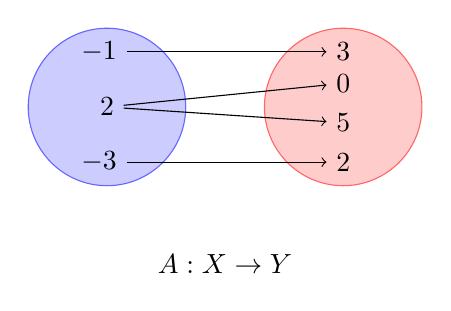
\begin{tikzpicture}
    % draw the sets
    \filldraw[fill=blue!20, draw=blue!60] (-1.5,0) circle (1cm);
    \filldraw[fill=red!20, draw=red!60] (1.5,0) circle (1cm);


    % the texts
    \node at (0,-2) {$A: X \to Y$};

    % the points in the sets (here I just create nodes to use them later on to position
    % the circles and the arrows
    \node (x1) at (-1.6,0.7) {$-1$};
    \node (x2) at (-1.5,0) {$2$};
    \node (x3) at (-1.6,-0.7) {$-3$};
    \node (y1) at (1.5,0.7) {$3$};
    \node (y2) at (1.5,0.3) {$0$};
    \node (y3) at (1.5,-0.2) {$5$};
    \node (y4) at (1.5,-0.7) {$2$};

    % draw the arrows
    \draw[->] (x1) -- (y1);
    \draw[->] (x2) -- (y2);
    \draw[->] (x2) -- (y3);
    \draw[->] (x3) -- (y4);

\end{tikzpicture}
\end{center}
% ============== SECTION
\section{Functions}
A function is actually a special kind of relation because it follows an extra rule. Just like a relation, a function is also a set of ordered pairs; however, \textsl{every $x$-value must be associated to only one $y$-value}.\\
For instance, consider the relation $A$. This relation is not a function since we have repetitions or duplicates of $x$-values with different $y$-values, then this relation ceases to be a function.
\begin{equation*}
    A =\{(-1,\,3),\,(\circled{2},\,0),\,(\circled{2},\,5),\,(-3,\,2)\} \quad \text{\xmark}
\end{equation*}
% ======== EXAMPLE 1
\begin{exa}
Determine whether each relation is a function.
    \begin{enumerate}[(a)]
       \item $S=\{(1,2),(3,4),(5,6),(5,8)\}$
        \item $T=\{(1,2),(3,4),(6,5),(8,5)\}$
    \end{enumerate}
\end{exa}
(a) As you can see number 5 in domain corresponds to both number 6 and 8. Since number 5 in the domain corresponds to more than one element in range, the relation $S$ is not a function.
\begin{equation*}
    S = \{(1,2),(3,4),(\circled{5},6),(\circled{5},8)\} \quad \text{\xmark}
\end{equation*}
This relation is also shown in Figure \eqref{fig:set_S}.\\
\begin{figure}[ht]
\centering
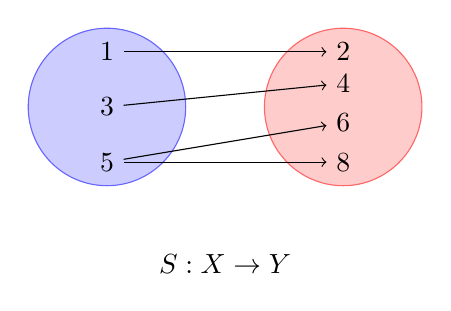
\begin{tikzpicture}
    % draw the sets
    \filldraw[fill=blue!20, draw=blue!60] (-1.5,0) circle (1cm);
    \filldraw[fill=red!20, draw=red!60] (1.5,0) circle (1cm);


    % the texts
    \node at (0,-2) {$S: X \to Y$};

    % the points in the sets (here I just create nodes to use them later on to position
    % the circles and the arrows
    \node (x1) at (-1.5,0.7) {$1$};
    \node (x2) at (-1.5,0) {$3$};
    \node (x3) at (-1.5,-0.7) {$5$};
    \node (y1) at (1.5,0.7) {$2$};
    \node (y2) at (1.5,0.3) {$4$};
    \node (y3) at (1.5,-0.2) {$6$};
    \node (y4) at (1.5,-0.7) {$8$};

    % draw the arrows
    \draw[->] (x1) -- (y1);
    \draw[->] (x2) -- (y2);
    \draw[->] (x3) -- (y3);
    \draw[->] (x3) -- (y4);

\end{tikzpicture}
\caption{Mapping diagram of relation $S$}
\label{fig:set_S}
\end{figure}

(b) In this relations, every element in the domain corresponds to exactly one element in the range. Therefore, the relation $T$ is a function. The mapping diagram of relation $T$ is shown below.\\
\begin{figure}[ht]
\centering
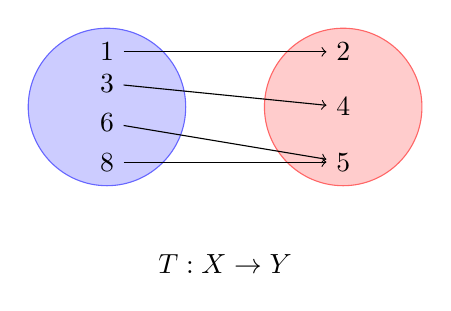
\begin{tikzpicture}
    % draw the sets
    \filldraw[fill=blue!20, draw=blue!60] (-1.5,0) circle (1cm);
    \filldraw[fill=red!20, draw=red!60] (1.5,0) circle (1cm);


    % the texts
    \node at (0,-2) {$T: X \to Y$};

    % the points in the sets (here I just create nodes to use them later on to position
    % the circles and the arrows
    \node (x1) at (-1.5,0.7) {$1$};
    \node (x2) at (-1.5,0.3) {$3$};
    \node (x3) at (-1.5,-0.2) {$6$};
    \node (x4) at (-1.5,-0.7) {$8$};
    \node (y1) at (1.5,0.7) {$2$};
    \node (y2) at (1.5,0) {$4$};
    \node (y3) at (1.5,-0.7) {$5$};

    % draw the arrows
    \draw[->] (x1) -- (y1);
    \draw[->] (x2) -- (y2);
    \draw[->] (x3) -- (y3);
    \draw[->] (x4) -- (y3);

\end{tikzpicture}
\caption{Mapping diagram of relation $T$}
\end{figure}
% ====== SUBSECTION
\subsection{Functions as equations}
Functions are usually given in terms of equations rather than as sets of of ordered pairs. Examples of several functions are below:
\begin{align*}
    y&=0.01x^2-0.2x+8.7\\
    y&= -2.9x+286\\
    y&=\sqrt{x-3}\\
    y&=\frac{x-1}{x+1} \\
    \vdots&
\end{align*}
A function is much like a machine, where you drop some random stuff in and the machine provides you with something else-much like a candy or chip machine where you input coins and you get out a tasty snack.
\begin{figure}[ht]
    \centering
    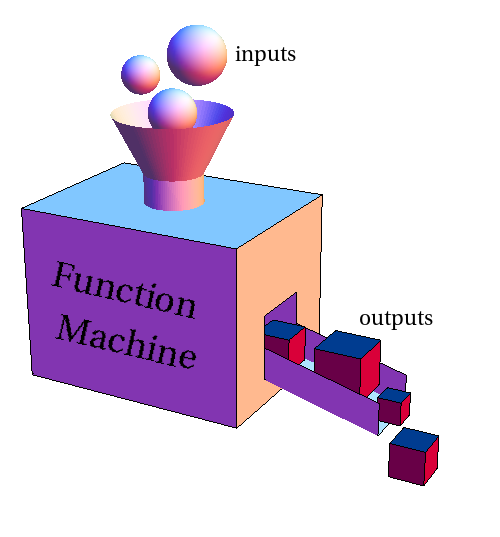
\includegraphics[width=6cm]{Pics/func_machine.png}
    \caption{Function as a machine}
    \label{fig:func_mach}
\end{figure}
\newpage
The function has has an input, $x$-value and an output, $y$-value. For each value of $x$, there is one and only one value of $y$. For this reason $x$ is considered as \textbf{an independent variable} and $y$ is considered as \textbf{dependent variable}.\\

% ======== SUBSECTION
\subsection{Vertical line test}
A great way to determine whether an equation is a function is looking at its graph. Because $x$ values are vertical lines we will draw a vertical line through the
graph. If the vertical line crosses the graph more than once, that means we have too many possible $y$ values. If the graph crosses the graph only once, then we say the equation represent a function.
% ============ EXAMPLE
\begin{exa}
    Use the vertical line test to identify  graphs in  which $y$ is a function of $x$.
\end{exa}
%
\begin{figure}[ht]
\centering
\subfloat[]{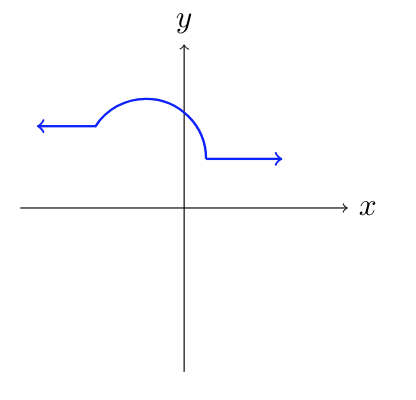
\includegraphics[width = 1in]{Pics/1.png}} 
\subfloat[]{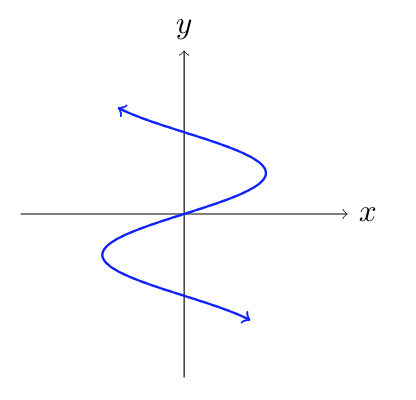
\includegraphics[width = 1in]{Pics/2.png}}
\subfloat[]{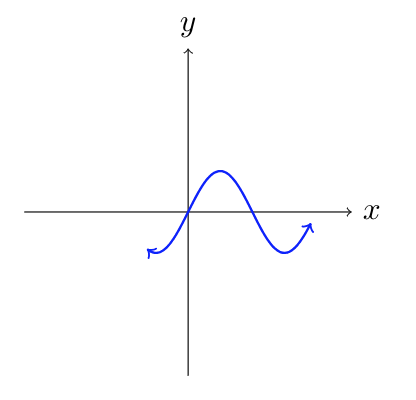
\includegraphics[width = 1in]{Pics/3.png}}
\subfloat[]{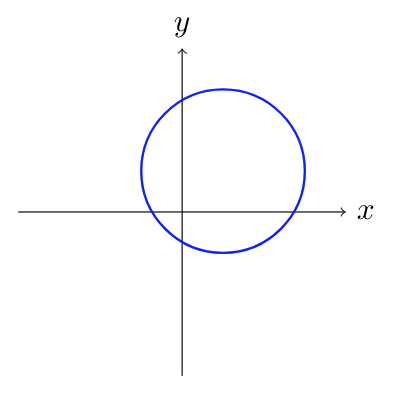
\includegraphics[width = 1in]{Pics/4.png}} 
\end{figure}
%
\noindent\begin{minipage}{0.4\textwidth}% adapt widths of minipages to your needs
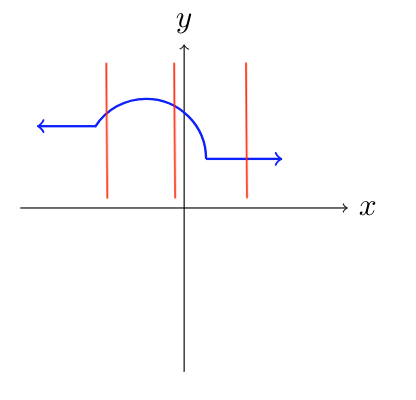
\includegraphics[width=\linewidth]{Pics/1_line.png}
(a) $y$ is a \textbf{function} of $x$.
\end{minipage}%
\hfill%
\begin{minipage}{0.4\textwidth}
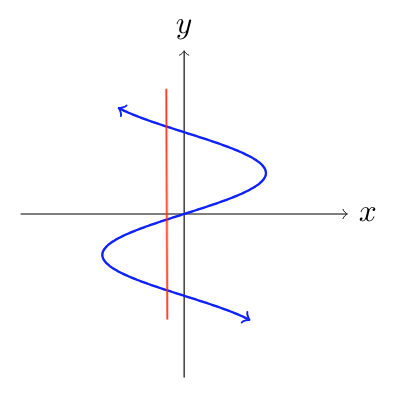
\includegraphics[width=\linewidth]{Pics/2_line.png}
(b) $y$ \textbf{is not a function} of $x$. Because a vertical line hit the graphs more than once.
\end{minipage}
%
\noindent\begin{minipage}{0.4\textwidth}% adapt widths of minipages to your needs
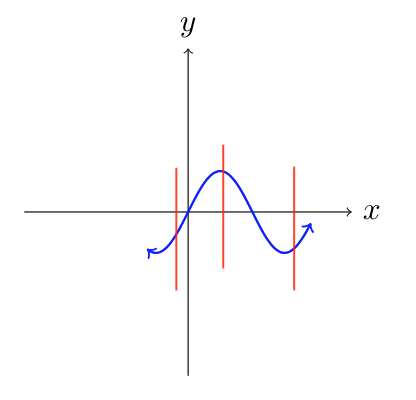
\includegraphics[width=\linewidth]{Pics/3_line.png}
(c) $y$ is a \textbf{function} of $x$.
\end{minipage}%
\hfill%
\begin{minipage}{0.4\textwidth}
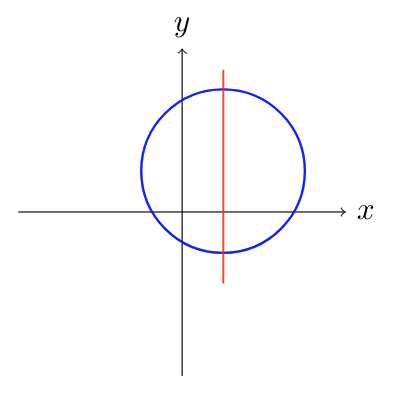
\includegraphics[width=\linewidth]{Pics/4_line.png}
(d) $y$ \textbf{is not a function} of $x$. Because a vertical line hit the graphs more than once.
\end{minipage}
%
% ======= SubSECTION
\subsection{Function Notation}
Often we will change the notation used to
emphasis the fact that it is a function. Instead of writing $y =$, we will use function notation which can be written $f(x) = $. We read this notation “$f$ of $x$”. Consider the function $y=x^2-4$. In function notation, we write it as $f(x)=x^2-4$.
\begin{nt}
It is important to point out that $f(x)$ does not mean
$f$ times $x$, it is merely a notation that names the function with the first letter (function $f$) and then in parenthesis we are given information about what variables
are in the function (variable $x$). The first letter can be anything we want it to be, often you will see $g(x)$ (read $g$ of $x$).
\end{nt}
% =========== SUBSECTION
\subsection{Evaluate a function}
To evaluate a function, $f(x)$, we need to substitute the specified input values for $x$ in the function's equation. This is shown in the following examples.
% ======= EXAMPLE 
\begin{exa}
    If $f(x)=x^2-2x+7$, evaluate each of the following:
    \begin{multicols}{3}
    \begin{enumerate}[a.]
        \item $f(-5)$
        \item $f(x+4)$
        \item $f(-x)$
    \end{enumerate}
    \end{multicols}
\end{exa}

\begin{align*}
    f(-5)=?&  &   &\text{Replace $x$ with -5}\\
    \textcolor{red}{(-5)}^2-2\textcolor{red}{(-5)}+7& &   &\text{Simplify}\\
    25+10+7&    &   &\text{Add}\\
    42& &   &\text{Our solution to part a}\\
    &   &   &\\
    f(x+4)=?&     &   &\text{Replace $x$ with $x+1$}\\
    \textcolor{red}{(x+4)}^2-2\textcolor{red}{(x+4)}+7& &   &\text{Simplify}\\
    x^2+16+8x-2x-8+7&   &   &\text{Combine like term}\\
    x^2+6x+17&  &   &\text{Our solution to part b}\\
    &   &   &\\
    f(-x)=?&  &   &\text{Replace $x$ with $-x$}\\
    \textcolor{red}{(-x)}^2-2\textcolor{red}{(-x)}+7& &   &\text{Simplify}\\
    x^2+2x+7&   &   &\text{Our solution to part c}
\end{align*}
% =======SECTION
\section{Obtaining information from a graph}
At the right or left of a graph you will see closed dots, open dots or arrows:
\begin{itemize}
    \setlength\itemsep{0em}
    \item A closed dot indicate that the graph does not extend beyond this point and the point itself \textbf{belongs} to the graph.
    \item An open dot indicate that the graph does not extend beyond this point and the point itself \textbf{does not belong} to the graph.
    \item An arrow indicate that the graph extend indefinitely in the direction which the arrows points.
\end{itemize}
\begin{figure}[ht]
    \centering
    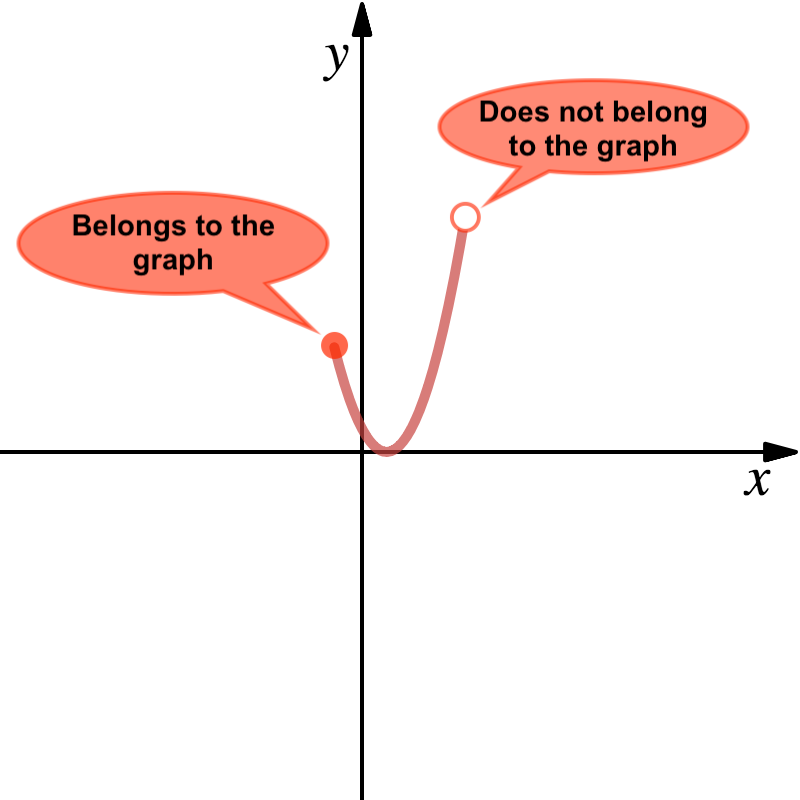
\includegraphics[width=4.2cm]{Pics/endpoints.png}
    \label{fig:endpoints}
\end{figure}


To evaluate a function at a given point, we must locate the point on the $x$-axis first. Then we draw a vertical line, to find the corresponding $y$-coordinate on the graph.
%============ EXAMPLE 4
\begin{exa}
    Given the graph, find $f(1)$.
\end{exa}
\begin{center}
\begin{tikzpicture}[scale=0.45]
\begin{axis}[my style, 
        minor tick num=1,
        xmin=-6,xmax=6,ymin=-26,ymax=26, samples=100]
  \addplot +[<->, mark=none, blue, ultra thick, domain=-3.5:3.5] (x,x*x*x-6*x);
\end{axis}
\end{tikzpicture}
\end{center}
To find $f(1)$ locate $x=1$ on the $x$-axis. Then we draw a vertical line to hit the graph to find the corresponding $y$-coordinate. We see that $y$-coordinate is $-5$. Therefore, $f(1)=-5$.
\begin{center}
\begin{tikzpicture}[scale=0.55]
\begin{axis}[my style, 
        minor tick num=1,
        xmin=-6,xmax=6,ymin=-26,ymax=26, samples=100]
  \addplot +[<->, mark=none, blue, ultra thick, domain=-3.5:3.5] (x,x*x*x-6*x);
  \addplot [dashed, red, thick] (1,x);
  \addplot [dashed, red, thick,domain=0:1] (x,-5);
  \node[draw=none,red] at (-0.5, -5)  ()  {$-5$};
    \node[draw=none,red] at (1.3, 1)  ()  {$1$};
\end{axis}
\end{tikzpicture}
\end{center}
% ========== SECTION
\section{Identifying domain and range from a graph}
To find the domain from a graph, compress (projecting) the graph onto the $x$-axis and see which values will be covered.  Similarly, to find the range using the graph of a function, compress (project) the graph onto the $y$-axis. We can use set-builder notation or interval notation to express the domain or range of a function.
% ====== EXAMPLE 5
\begin{exa}
    Use the graph of each function to identify its domain and its range.
\end{exa}

\vspace{-0.4cm}
\begin{figure}[ht]
\centering
\subfloat[]{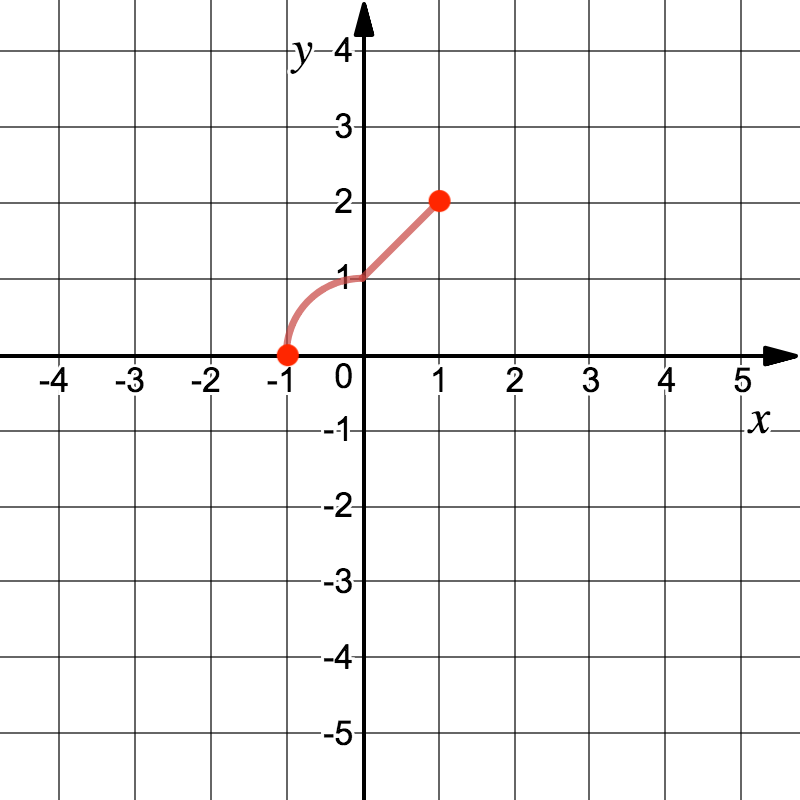
\includegraphics[width = 1.3in]{Pics/ex4_a.png}}
 \qquad
\subfloat[]{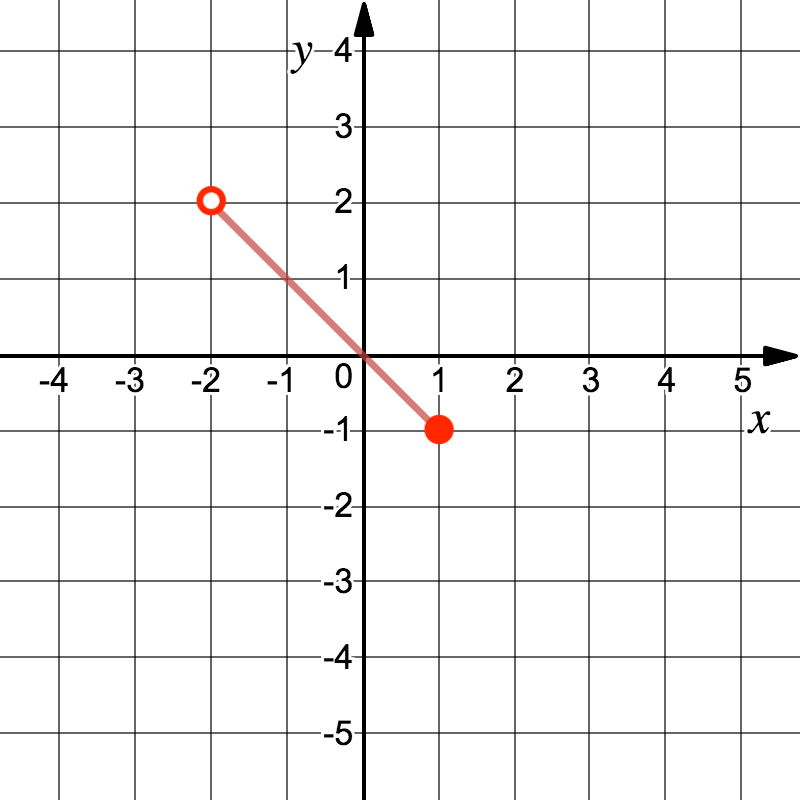
\includegraphics[width = 1.3in]{Pics/ex4_b.png}}
 \qquad
\subfloat[]{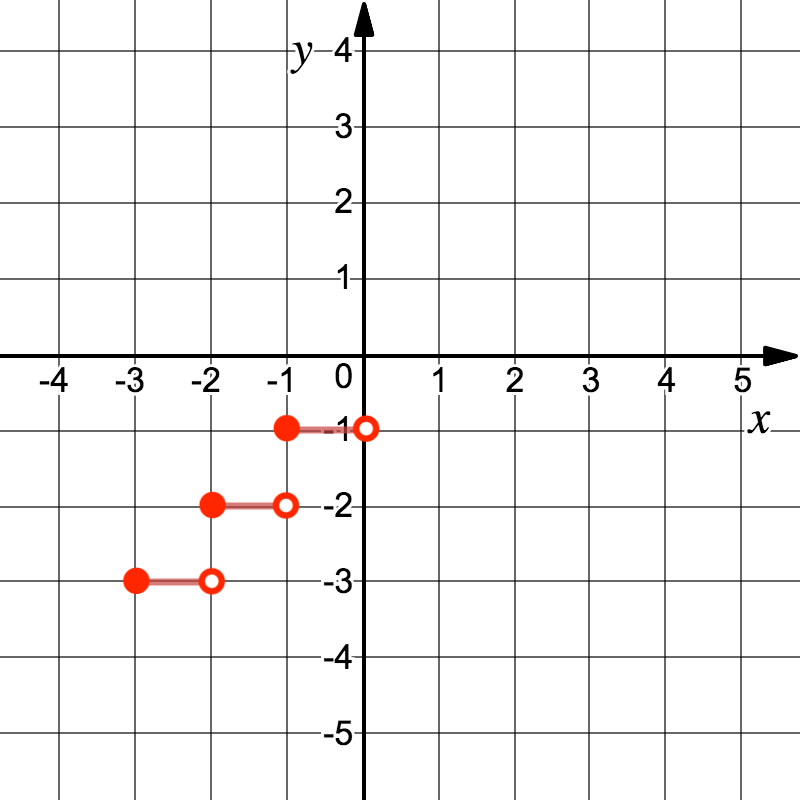
\includegraphics[width = 1.3in]{Pics/ex4_c.png}}
\end{figure}
%%%% ANS
\noindent\begin{minipage}{0.4\textwidth}% adapt widths of minipages to your needs
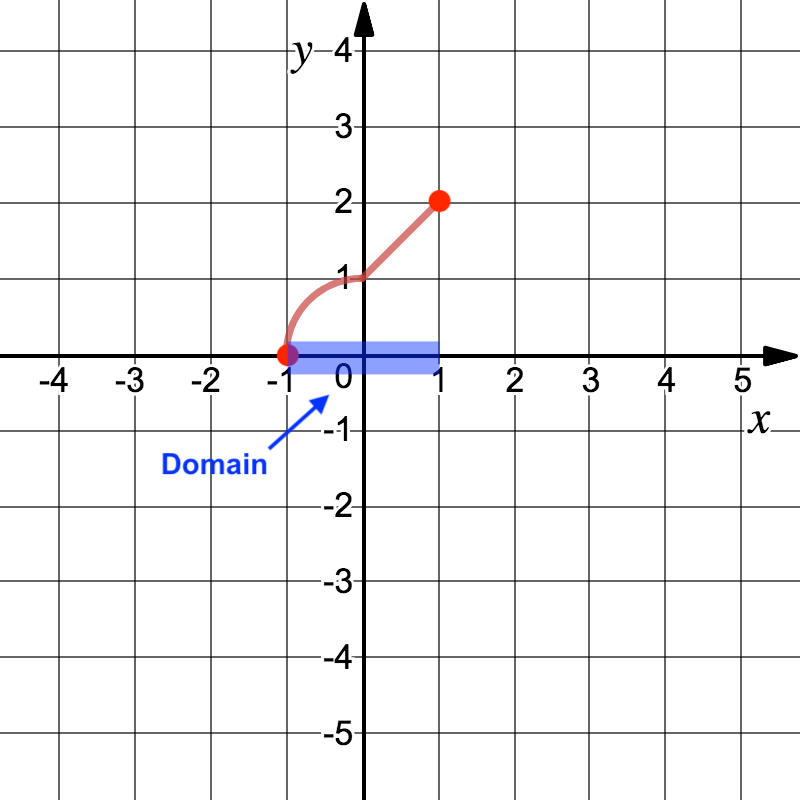
\includegraphics[width=\linewidth]{Pics/ex4_a_D.png}
(a) Domain :\\ $[-1,1]$ or $\{x \mid -1 \le x \le 1\}$
\end{minipage}%
\hfill%
\begin{minipage}{0.4\textwidth}
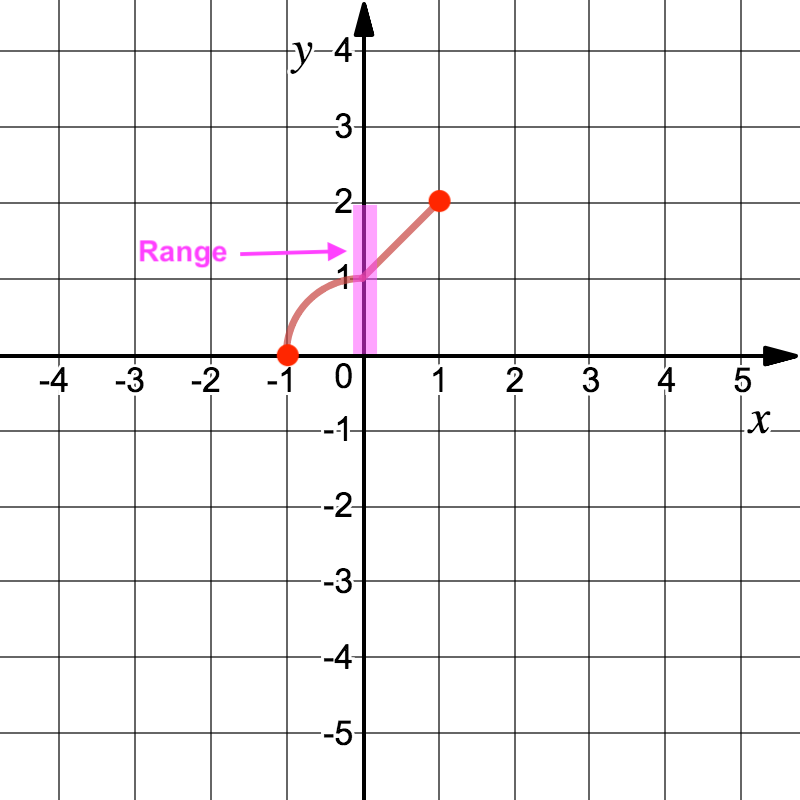
\includegraphics[width=\linewidth]{Pics/ex4_a_R.png}
Range:\\ $[0,2]$ or $\{y \mid 0 \le y \le 2\}$
\end{minipage}
%


\vspace{0.4cm}
\noindent\begin{minipage}{0.4\textwidth}% adapt widths of minipages to your needs
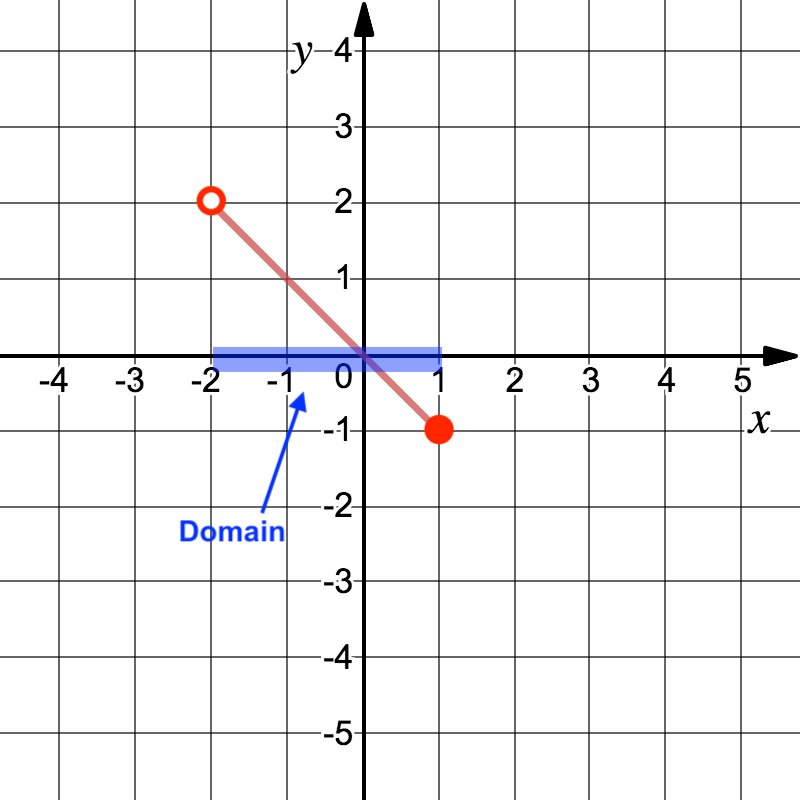
\includegraphics[width=\linewidth]{Pics/ex4_b_D.png}
(b) Domain :\\ $(-2,1]$ or $\{x \mid -2 < x \le 1\}$
\end{minipage}%
\hfill%
\begin{minipage}{0.4\textwidth}
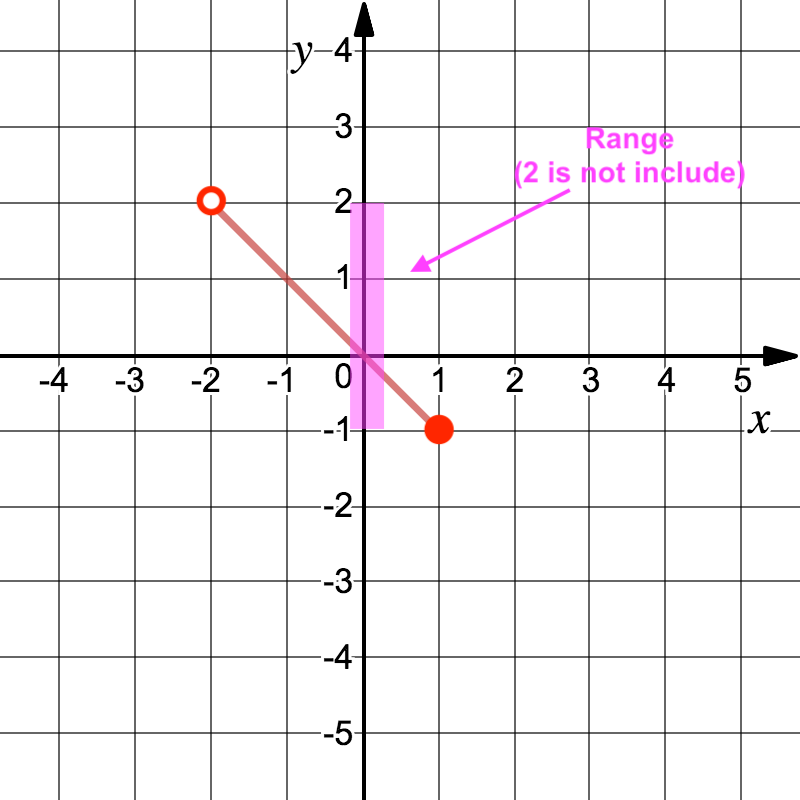
\includegraphics[width=\linewidth]{Pics/ex4_b_R.png}
Range:\\ $[-1,2)$ or $\{y \mid -1 \le y < 2\}$
\end{minipage}
%


\vspace{0.4cm}
\noindent\begin{minipage}{0.4\textwidth}% adapt widths of minipages to your needs
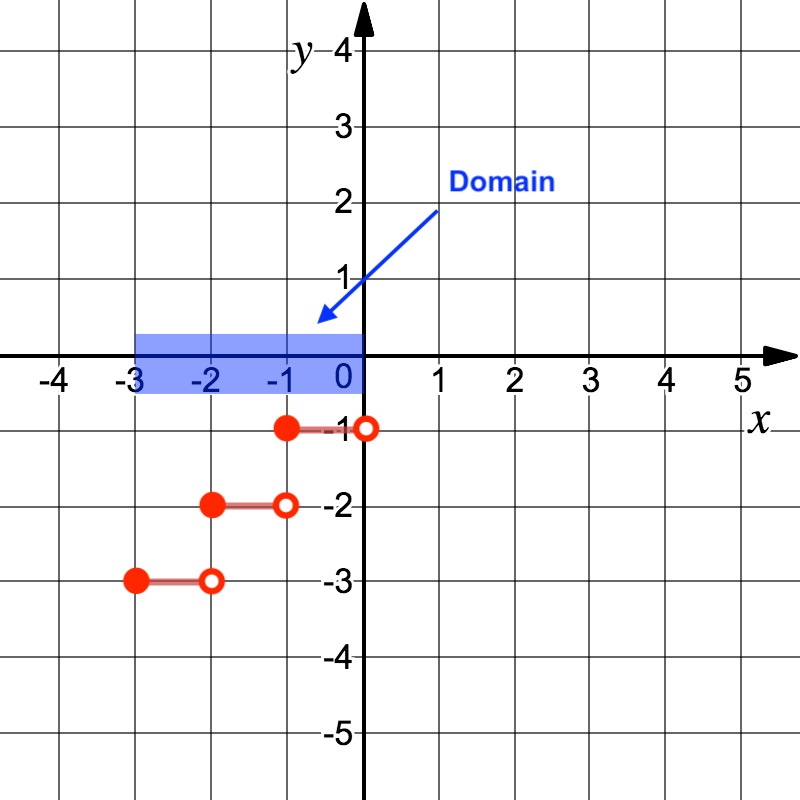
\includegraphics[width=\linewidth]{Pics/ex4_c_D.png}
(c) Domain :\\ $[-3,0)$ or $\{x \mid -3 \le x < 0\}$
\end{minipage}%
\hfill%
\begin{minipage}{0.4\textwidth}
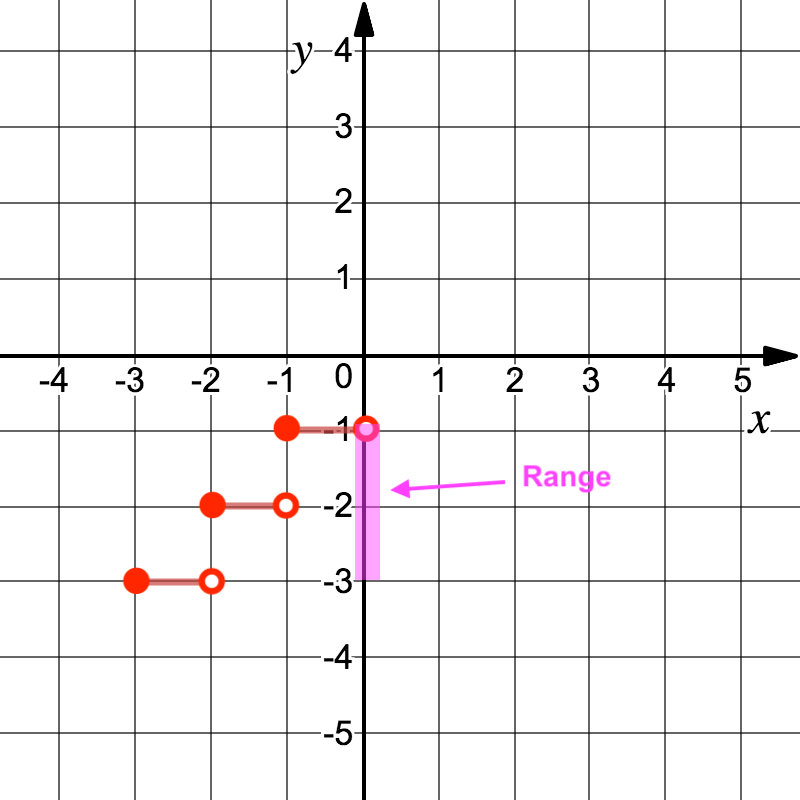
\includegraphics[width=\linewidth]{Pics/ex4_c_R.png}
Range:\\ $[-3,-1]$ or $\{y \mid -3 \le y \le -1\}$
\end{minipage}